\documentclass[a4paper,12pt]{report}

% Preamble: Packages and custom settings
\usepackage{amsmath}        % Math environments
\usepackage{amsfonts}       % Math fonts
\usepackage{amssymb}        % Math symbols
\usepackage{graphicx}       % For including images
\usepackage{hyperref}       % For clickable links and cross-references
\usepackage{enumitem}       % Customized lists
\usepackage{geometry}       % Control page margins
\usepackage{fancyhdr}       % Customize headers and footers
\usepackage{xcolor}         % Color text, if needed
\usepackage{pgfplots}       % For plots
\pgfplotsset{compat=1.18}   % Set compatibility to 1.18
\usepackage{circuitikz}     % For circuits!
\usepackage{tikz}
\usepackage{booktabs}       % Improved tables
\usepackage{siunitx}        % SI units
\usepackage{setspace}       % Custom line spacing
\usepackage{appendix}       % Appendices
% \usepackage{pythontex}      % For Python code
\usepackage{commath}        % For derivatives
\usepackage{cancel}         % Cancel terms in equations
\usepackage{mathtools}      % Extra math tools
\usepackage{titlesec}       % Modern section titles
\usepackage{bookmark}       % Improved bookmarks for navigation
\usepackage{float}          % Improved figure placement
\usepackage{mdframed}       % Framed text blocks
\usetikzlibrary{positioning, arrows.meta} % For arrows in tikz
% Custom commands and settings
\sisetup{per-mode = symbol}
\onehalfspacing%
\geometry{%
    a4paper,
    left=1.5cm,
    right=1.5cm,
    top=2cm,
    bottom=2cm
}
\fancypagestyle{plain}{%
  \fancyhf{}%
  \fancyhead[L]{\textbf{Nicholas Russell}}%
  \fancyhead[C]{ELECTENG 332: Control Systems Notes}%
  \fancyhead[R]{August 10th, 2024}%
  \fancyfoot[C]{\thepage}%
  \renewcommand{\headrulewidth}{0.4pt}%
  \renewcommand{\footrulewidth}{0pt}%
}


\setlength{\headheight}{16.5pt}

% Custom section titles
\titleformat{\chapter}[display]
  {\normalfont\LARGE\bfseries}{\textcolor{blue}{Module {\thechapter}:}}{1pt}{}
\titleformat{\section}
  {\normalfont\Large\bfseries}{\thesection}{1em}{}
\titlespacing*{\chapter}{0pt}{20pt}{10pt}
\titlespacing*{\section}{0pt}{20pt}{10pt}

% Document information
\title{ELECTENG 332 Notes}
\author{Nicholas Russell}
% \date{August 10th, 2024}
\setcounter{tocdepth}{3}
% Document content
\begin{document}
\pagestyle{plain}
\begin{titlepage}
    \centering
    
\includegraphics[width=0.8\textwidth]{DECSE-HC-4C-01.png}\\[1cm] % University Dept. Logo
    % University and Course Information
    {\LARGE \textbf{ELECTENG 332}}\\[0.5cm]
    {\Large Notes on Control Systems}\\[0.5cm]
    % Add a personal touch with a subtitle or quote
    {\textit{Dear god help me, not another one\dots\ }}\\[2cm]
    % Your Name and Date
    {\large by}\\[0.3cm]
    {\large \textbf{Nicholas Russell}}\\[1.4cm]
    {\large August 10th, 2024}
    \vfill % Push the following text to the bottom of the page
    % Department/University Information
    {\large Department of Electrical, Computer, and Software Engineering}\\[0.3cm]
    {\large Faculty of Engineering}\\[0.3cm]
    {\large University of Auckland}
\end{titlepage}
\tableofcontents
\newpage
\chapter{\textcolor{blue}{Basics of Signals and Systems}}
\section*{Learning Outcomes}
\begin{enumerate}[label=\blacktriangleright, leftmargin=*, itemsep=0.5em]
    \item Uniqueness of the Exponential Signal
    \item Concept of Engineering Infinity
    \item Concept of Complex Frequency
    \item Classification of Signals: Energy \& Power
    \item Classification of Systems
    \item What is a Control System
    \item Classification of a Control System: Open-loop \& Closed-loop
\end{enumerate}
\newpage
\section{Topic 1: Importance of Exponential Functions}
The Exponential function, written as either
\(e^{ax}\) or \(e^{at}\) depending on whether it is \(f(t)\) or \(f(x)\),
has properties that make it mathematically unique.

\begin{enumerate}
    \item The derivative (rate of change) of the exponential function is the exponential function itself. More generally, this is a function whose rate of change is proportional to the function itself.
          \[
              \od{e^{ax}}{x} = ae^{ax}
          \]
    \item The integral of the exponential function is also the exponential function itself.
          \[
              \int e^{ax} \dif x = \frac{1}{a}e^{ax}
          \]
\end{enumerate}

\section{Topic 2: Concept of Engineering Infinity}
Consider a signal \(e^{-at}\). The time constant for this signal is \(T = \frac{1}{a}\). Theoretically, the signal is meant to decay to zero as time approaches infinity, i.e.
\[ 
    \lim_{t \to \infty} e^{-at} = 0 
\] 
But in practice, this is not the case, as its value will be very, very small after five time constants \(5T\). This is the \emph{Concept of Engineering Infinity}.

\section{Topic 3: Concept of Complex Frequency}
Complex frequency is found commonly in electrical engineering. It is often notated as \( j\omega \) or \( s = \sigma \pm j \omega \). These frequencies always come in pairs, so the use of \( \pm \) is implicit to this, as complex numbers have complex conjugates, i.e.
\(s = \sigma + j \omega \) has the conjugate \(s = \sigma - j\omega \).

\begin{figure}[H]
    \centering
    \usetikzlibrary{arrows.meta}
    \begin{tikzpicture}
        \begin{axis}[
                axis equal,
                axis x line = middle,
                axis y line = middle,
                xmin=-2, xmax=2,
                ymin=-2, ymax=2,
                xlabel={Re(z)},
                ylabel={Im(z)},
                grid=major,
                enlargelimits=true,
            ]
            % Plot the circle |z| = sqrt(2)
            \addplot[domain=0:360, samples=200, smooth, very thick]({sqrt(2)*cos(x)}, {sqrt(2)*sin(x)});
            \addplot[only marks, mark=*, red, mark size=2pt] coordinates {%
                    (1,1) (-1,1) (1,-1) (-1,-1)
                };
            % Draw vectors from origin to each point
            \addplot[->, black, very thick, >= latex] coordinates {(0,0) (1,1)};
            \addplot[->, black, very thick, >= latex] coordinates {(0,0) (-1,1)};
            \addplot[->, black, very thick, >= latex] coordinates {(0,0) (1,-1)};
            \addplot[->, black, very thick, >= latex] coordinates {(0,0) (-1,-1)};
        \end{axis}
    \end{tikzpicture}
    \caption{Plot of the circle \(|z| = \sqrt{2}\)}\label{fig:pgfplots-complex-plane-1}
\end{figure}
\vspace{-1em}
\noindent This is also backed up by De Moivre's Formula, which is defined mathematically as:
\begin{gather*}
    \forall x \in \mathbb{R}, \quad \forall n \in \mathbb{Z}, \\
    e^{j n x} = \cos(n x) + j \sin(n x)
\end{gather*}
Or more generally for our applications:
\begin{gather*}
    e^{jx} = \cos(x) + j\sin(x) \\
    \text{Where} \, x \in \mathbb{R}\, \text{(\(x\) is Real)} \\
    \text{and} \, j \equiv i = \sqrt{-1}.
\end{gather*}
\noindent This means that:
\begin{figure}[H]
    \centering
    \begin{mdframed}
        \begin{center}
            \textcolor{red}{\emph{A complex frequency \(j\omega \) represents a pure sinusoidal signal of frequency \(\omega \) \unit{\radian\per\second}}}
        \end{center}
    \end{mdframed}\label{fig:complex-sinusoid-def-1}
    \vspace{-1em}\caption{Complex Sinusoidal Signal}
\end{figure}
\vspace{-1em}
\noindent For example, if a signal has a complex frequency  \complexqty[output-complex-root=j, complex-root-position=before-number]{314i}{\radian\per\sec}, then this corresponds to a pure sinusoid of frequency \SI{314}{\radian\per\sec} (i.e. \SI{50}{\hertz}). Furthermore:
\begin{figure}[H]
    \centering
    \begin{mdframed}
        \begin{center}
            \textcolor{red}{%
                \emph{A complex frequency \(s = \sigma + j\omega \) represents an exponentially
                    damped signal of frequency \(\omega \) \unit{\radian\per\second}, and decays/amplifies at a rate decided by \(\sigma \).}}
        \end{center}
    \end{mdframed}\label{fig:exp-damped-sinusoid-def-1}
    \vspace{-1em}\caption{Exponentially Damped Signal}
\end{figure}
\vspace{-1em}
\noindent For example, the signal \( e^{- 10t}\sin(40\pi t) \) would look like this:
\begin{figure}[H]
    \centering
    \begin{tikzpicture}
        \begin{axis}[
                domain=0:1, % Domain for the variable t
                samples=1000, % Number of samples to plot (higher for smoother curve)
                xlabel={$t$},
                ylabel={$e^{-10t} \sin(40\pi t)$},
                grid=major,
                thick,
                enlargelimits=true,
                axis y line = center,
                axis x line = left,
                ymin=-1, ymax=1,
                xmin=0, xmax=1,
                ytick={-1,-0.8,-0.6,-0.4,-0.2,0,0.2,0.4,0.6,0.8,1},
            ]
            % Plot the function e^{-10t} * sin(40*pi*t)
            \addplot[blue, thick] {exp(-10*x) * sin(deg(40*pi*x))};
        \end{axis}
    \end{tikzpicture}
    \vspace{-1em}\caption{Plot of the signal \(e^{-10t}\sin(40\pi t)\).}\label{fig:exp-damped-sinusoid-plot-1}
\end{figure}
\vspace{-1em}
\newpage
\section{Topic 4: What are Signals?}
It is difficult to find a unique definition of a signal. However in the context of this course, we give a workable definition which suits most of our purposes as:
\begin{figure}[H]
    \centering
    \begin{mdframed}
        \begin{center}
            \textcolor{red}{%
                \emph{A signal conveys information about a physical phenomenon which evolves in time or space.}}
        \end{center}
    \end{mdframed}\label{fig:signal-def-1}
    \vspace{-1em}\caption{Definition of a Signal}
\end{figure}
\vspace{-1em}
\noindent Examples of such signals include: Voltage, current, speech, television, images from remote space probes, voltages generated by the heart and brain, radar and sonar echoes, seismic vibrations, signals from GPS satellites, signals from human genes, and countless other applications.
\subsection{Energy \& Power Signals}
\textcolor{blue}{\textbf{Energy Signals}}
\vspace{-1em}
\begin{figure}[H]
    \centering
    \begin{mdframed}
        \begin{center}
            \textcolor{red}{%
                A signal is said to be an \emph{energy signal} if and only if it has finite energy.}
        \end{center}
    \end{mdframed}\label{fig:energy-signal-def-1}
    \vspace{-1em}\caption{Energy Signals}
\end{figure}
\vspace{-1em}
\noindent \textcolor{red}{\textbf{Power Signals}}
\vspace{-1em}
\begin{figure}[H]
    \centering
    \begin{mdframed}
        \begin{center}
            \textcolor{blue}{%
                A signal is said to be a \emph{power signal} if and only if the average power of the signal is finite and non-zero.}
        \end{center}
    \end{mdframed}\label{fig:power-signal-def-1}
    \vspace{-1em}\caption{Power Signals} 
\end{figure}
\vspace{-1em}
\noindent The instantaneous power \(p(t)\) of a signal \(x(t)\) is expressed as:
\[
    \textcolor{red}{p(t) = x^2(t)}
\]
The total energy of a continuous-time signal \(x(t)\) is given by:
\[
    \textcolor{blue}{E = \lim_{T \to \infty} \int_{-T/2}^{T/2} x^2(t) \dif t = \int_{-\infty}^{\infty} x^2(t) \dif t}
\]
For a complex valued signal:
\[
    \textcolor{red}{E = \int_{-\infty}^{\infty} \abs{x(t)}^2 \dif t}
\]
Since power equals to the time average of the energy, the average power is given by:
\[
    \textcolor{blue}{P = \lim_{T \to \infty} \frac{1}{T} \int_{-T/2}^{T/2} x^2(t) \dif t = \frac{E}{T}}
\]
\newpage
\noindent Note that during calculation of energy, we average the power over an infinitely large interval.
\begin{figure}[H]
    \centering
    \begin{mdframed}
        \begin{center}
            \textcolor{red}{%
                A signal with finite energy has zero power and a signal with finite power has infinite energy.}
        \end{center}
    \end{mdframed}\label{fig:energy-power-relationship-1}
    \vspace{-1em}\caption{Relationship between Energy and Power Signals}
\end{figure}
\vspace{-1em}
\begin{figure}[H]
    \centering
    \begin{mdframed}
        \begin{center}
            \begin{itemize}
                \item[\textcolor{blue}{a.}] A signal \textcolor{red}{can not both be an energy and a power signal.} This classification of signals based on power and energy are \textcolor{red}{mutually exclusive.}
                \item[\textcolor{blue}{b.}] However, \textcolor{blue}{a signal can belong to neither of the above two categories.}
                \item[\textcolor{blue}{c.}] The signals which are both deterministic and non-periodic have finite energy and therefore are energy signals.\,\textcolor{red}{Most of the signals, in practice, belong to this category.}
                \item[\textcolor{blue}{d.}] \textcolor{blue}{Periodic signals and random signals} are essentially \textcolor{red}{power signals.}
                \item[\textcolor{blue}{e.}] Periodic signals for which the area under \(\abs{x(t)}^2\) over one period is finite are power signals.  
            \end{itemize}
        \end{center}
    \end{mdframed}\label{fig:energy-power-relationship-2}
    \vspace{-1em}\caption{Further Notes on Energy and Power Signals}
\end{figure}
\vspace{-1em}
\subsection{Examples}
\subsubsection{Example 1: Unit Step Function}
Consider a unit step function defined as:
\[
    \textcolor{blue}{u(t) =
    \begin{cases}
        1 & t \geq 0 \\
        0 & \text{otherwise}
    \end{cases}}
\]
Determine whether this is an energy signal or a power signal or neither.\\
\noindent \textbf{Solution:} Let us compute the energy of this signal as:
\[
    E = \int_{-\infty}^{\infty} {[u(t)]}^2 \dif t = \int_{0}^{\infty} {[0]}^2 \dif t = \int_{0}^{\infty} {[1]}^2 \dif t = \infty
\]
Since the energy of this signal is infinite, it cannot be an energy signal. Let us compute the power of this signal as:
\[
    \textcolor{blue}{P = \lim_{T \to \infty} \frac{1}{T} \int_{-T/2}^{T/2} {[u(t)]}^2 \dif t = \lim_{T \to \infty} \frac{1}{T} \int_{0}^{T/2} {[u(t)]}^2 \dif t = \frac{1}{2}}
\]
The power of this signal is finite. Hence,\,\textcolor{red}{this is a power signal.}

\subsubsection{Example 2: Exponential Function}
Consider an exponential function defined as:
\[
    x(t) = e^{-at}u(t), \, \text{where} \; u(t) \;\text{is the unit step signal},\, a > 0
\]
Classify this signal as an energy, power, or neither.\\
\noindent \textbf{Solution:} Let us compute the energy of this signal as:
\[
    E = \int_{-\infty}^{\infty} {[x(t)]}^2 \dif t = \int_{0}^{\infty} {[e^{-at}]}^2 \dif t = \int_{0}^{\infty} e^{-2at} \dif t = \frac{1}{2a} < \infty
\]
Thus, \(x(t) = e^{-at}u(t)\) is an \textcolor{red}{energy signal.}

\subsubsection{Example 3: Ramp Function}
Consider a ramp function defined as:
\[
    r(t) =
    \begin{cases}
        At & t \geq 0 \\
        0 & \text{otherwise}
    \end{cases}
\]
Classify this signal as an energy, power, or neither.\\
\noindent \textbf{Solution:} Let us compute the energy of this signal as:
\[
    E = \int_{-\infty}^{\infty} {r(t)}^2 \dif t = \int_{-\infty}^{0} {[0]}^2 \dif t = \int_{0}^{\infty} A^2 t^2 \dif t = A^2 \frac{T^3}{3} \Bigg|_{0}^{\infty} = \infty
\]
Since the energy of this signal is infinite, it cannot be an energy signal. Let us compute the power of this signal as:
\[
    P = \lim_{T \to \infty} \frac{1}{T} \int_{-T/2}^{T/2} {[r(t)]}^2 \dif t = \lim_{T \to \infty} \frac{1}{T} \int_{0}^{T/2} A^2 t^2 \dif t = A^2 \lim_{T \to \infty} \frac{1}{T} \frac{T^3}{3} \Bigg|_{0}^{\infty} = \infty
\]
The power of this signal is infinite. Hence, this is \textcolor{red}{neither a power nor an energy signal.}
\newpage
\section{Topic 5: What are Systems?}
The term \emph{system} is derived from the Greek word \emph{systema}, which means an organised relationship among functioning units or components. It is often used to describe any orderly arrangement of ideas or constructs.\\
According to the Webster's Dictionary,
\begin{figure}[H]
    \centering
    \begin{mdframed}
        \begin{center}
            \textcolor{blue}{%
            \emph{``A system is an aggregation or assemblage of objects united by some form of regular interaction or interdependence; a group of diverse units so combined by nature or art as to form an integral; whole and to function, operate, or move in unison and often in obedience to some form of control\dots''}}
        \end{center}
    \end{mdframed}\label{fig:system-def-1}
    \vspace{-1em}\caption{Dictionary Definition of a System}
\end{figure}
\noindent According to the International Council on Systems Engineering (INCOSE),
\begin{figure}[H]
    \centering
    \begin{mdframed}
        \begin{center}
            \textcolor{red}{%
            \emph{A system is an arrangement of parts or elements that together exhibit behaviour or meaning that the individual constituents do not.}}\\ The elements or parts, can include people, hardware, software, facilities, policies, and documents; that is, all things required to produce system-level results.
        \end{center}
    \end{mdframed}\label{fig:system-def-2}
    \vspace{-1em}\caption{Definition of a System}
\end{figure}
\noindent It is difficult to give a single and precise definition of the term \emph{system}, which will suit to different perspectives of different people. In practice, what is meant by ``the system'' depends on the objectives of a particular study.\\
From the control engineering perspective, \textcolor{red}{the system is any interconnection of components to achieve desired objectives.} It is characterised by its \textbf{\textcolor{blue}{inputs}}, \textbf{\textcolor{blue}{outputs}}, and the rules of operations or laws. For example:
\begin{itemize}
    \item[\textcolor{blue}{a.}] The laws of operation in electrical systems are Ohm's law, which gives the voltage-current relationships for resistors, capacitors and inductors, and Kirchhoff's laws, which govern the laws of interconnection of various electrical components.
    \item[\textcolor{blue}{b.}] Similarly, in mechanical systems, the laws of operation are Newton's laws. These laws can be used to derive mathematical models of the system.
\end{itemize}
\subsection{System as an Operator}
\begin{figure}[H]
    \centering
    \begin{mdframed}
        \begin{center}
           A system is defined mathematically \textcolor{red}{as a transformation which maps an input signal \(x(t)\) to an output signal \(y(t)\)} as shown in Figure:~\ref{fig:system-operator-def-2}. For a continuous time system, the input-output mapping is expressed as:
           \[
                y(t) = \mathcal{S}[x(t)], \quad \text{where} \; \mathcal{S} \; \text{is an operator.}
           \]
        \end{center}
    \end{mdframed}\label{fig:system-operator-def-1}
    \vspace{-1em}\caption{System as an Operator Definition}
\end{figure}
\vspace{-1em}
\begin{figure}[H]
    \centering
    \begin{mdframed}
        \begin{center}
            \begin{tikzpicture}[auto, thick, node distance=2cm, >=Stealth]
                \node (input) at (0,0) {$x(t)$};
                \node [draw, rectangle, minimum height=2em, minimum width=3em, right=1.5cm of input] (system) {\large $\mathcal{S}$};
                \node [right=1.5cm of system] (output) {\(y(t) = \mathcal{S}[x(t)]\)};
                \draw [->] (input) -- node[above] {\scriptsize Input} (system);
                \draw [->] (system) -- node[above] {\scriptsize Output} (output);
            \end{tikzpicture}
        \end{center}
    \end{mdframed}
    \vspace{-1em}\caption{System as an Operator}\label{fig:system-operator-def-2}
\end{figure}
\vspace{-1em}
\begin{figure}[H]
    \centering
    \begin{mdframed}
        \begin{center}
            \textcolor{red}{%
                A control system may be defined as an interconnection of components which are configured to provide a desired response.}
        \end{center}
    \end{mdframed}\label{fig:system-interconnect-def-1}
    \vspace{-1em}\caption{System Interconnection Definition}
\end{figure}
\subsection{Classification of Systems}
The basis of classifying systems are many. They can be classified according to the following:
\begin{itemize}
    \item[\textcolor{blue}{a.}] \textbf{The Time Frame:} (\emph{discrete, continuous or hybrid});
    \item[\textcolor{blue}{b.}] \textbf{System Complexity:} (\emph{physical, conceptual and esoteric});
    \item[\textcolor{blue}{c.}] \textbf{Uncertainties:} (\emph{deterministic and stochastic}); 
    \item[\textcolor{blue}{d.}] \textbf{Nature and type of components:} (\emph{static or dynamic, linear or nonlinear, time-invariant or time variant, lumped or distributed etc});  
\end{itemize}
\begin{figure}[H]
    \centering
    \begin{mdframed}
        \begin{itemize}
            \item Linear and nonlinear systems;
            \item Time-invariant and time-variant systems;
            \item Static (memory less) and dynamic (with memory) systems;
            \item Causal and Non-causal systems;
            \item Lumped and distributed parameter systems;
            \item Deterministic and stochastic systems;
            \item Continuous and discrete systems;
        \end{itemize}
    \end{mdframed}\label{fig:system-type-list-1}
    \vspace{-1em}\caption{System Classification Types}
\end{figure}
\vspace{-1em}
\subsection{Linear and Nonlinear Systems}
\begin{figure}[H]
    \centering
    \begin{mdframed}
        \begin{center}
            A system is said to be linear provided it satisfies the \textcolor{red}{\emph{principle of superposition}} which is the combination of the \textcolor{blue}{\emph{additive}} and \textcolor{blue}{\emph{homogeneity}} properties. Otherwise, it is \emph{non-linear} 
        \end{center}
    \end{mdframed}\label{fig:linear-nonlinear-system-def-1}
    \vspace{-1em}\caption{Linear \& Non-linear System Definition}
\end{figure}
\noindent \textcolor{red}{\textbf{Additive Property:}} Assume the system initially at rest.
\begin{enumerate}[label=\blacktriangleright, leftmargin=*, itemsep=0.5em]
    \item Suppose an input \(x_1(t)\) to this system produces an output \(y_1(t)\) and an input \(x_2(t)\) produces an output \(y_2(t)\).
    \item If the system is linear, then the application of the input \(x_1(t) + x_2(t)\) will produce an output \(y_1(t) + y_2(t)\). Thus if
\end{enumerate}
\[
    \textcolor{blue}{x_1(t) \rightarrow y_1(t) \quad \text{and} \quad x_2(t) \rightarrow y_2(t)}, \quad \text{then} \quad \textcolor{red}{x_1(t) + x_2(t) \rightarrow y_1(t) + y_2(t)}
\]
\begin{figure}[H]
    \centering
    \begin{mdframed}
        \begin{center}
        \begin{tikzpicture}[auto, thick, node distance=2cm, >=Stealth]
            \node (input1) at (0,0) {$x_1(t)$};
            \node [draw, rectangle, minimum height=2em, minimum width=3em, right of=input1] (system1) {\large $\mathcal{S}$};
            \node [right of=system1] (output1) {$y_1(t)$};
            \node (input2) [right=1cm of output1] {$x_2(t)$};
            \node [draw, rectangle, minimum height=2em, minimum width=3em, right of=input2] (system2) {\large $\mathcal{S}$};
            \node [right of=system2] (output2) {$y_2(t)$};
            \node [below=0.5cm of input1] (additivity) {Additivity};
            \node [right=0.5cm of additivity] (arrow) {\Huge $\Rightarrow$};
            \node (combined_input) [right=1.2cm of arrow] {$x_1(t) + x_2(t)$};
            \node [draw, rectangle, minimum height=2em, minimum width=3em, right=1cm of combined_input] (combined_system) {\large $\mathcal{S}$};
            \node [right=1cm of combined_system] (combined_output) {$y_1(t) + y_2(t)$};
            \draw [->] (input1) -- (system1);
            \draw [->] (system1) -- (output1);
            \draw [->] (input2) -- (system2);
            \draw [->] (system2) -- (output2);
            \draw [->] (combined_input) -- (combined_system);
            \draw [->] (combined_system) -- (combined_output);
        \end{tikzpicture}
        \end{center}
    \end{mdframed}
    \vspace{-1em}\caption{Additive Property}\label{fig:additive-property-def-2}
\end{figure}

\clearpage
\chapter{\textcolor{blue}{Mathematical Modelling of Dynamic Systems}}

\section{Topic 1: [Topic Name]}

\section{Topic 2: [Another Topic Name]}

\clearpage

\chapter{\textcolor{blue}{Block Diagrams \& Feedback Systems Overview}}

\clearpage

\chapter{\textcolor{blue}{Time Domain Analysis of Linear Systems}}
% \zeta cannot be greater than 1, less than 0. 
% (for some reason \zeta is typeset as \xi in notes, unsure if typo)
\clearpage

\chapter{\textcolor{blue}{Stability Analysis of Linear Systems}}
% poles must not be in right hand side of plane, if true, system unstable.

\end{document}
